% ------------------------------------------------------------------------------
% TYPO3 CMS 7.3 - What's New - Chapter "Extbase & Fluid" (English Version)
%
% @author	Michael Schams <schams.net>
% @license	Creative Commons BY-NC-SA 3.0
% @link		http://typo3.org/download/release-notes/whats-new/
% @language	English
% ------------------------------------------------------------------------------
% LTXE-CHAPTER-UID:		ba9bf9d9-564d719b-a45c6394-358e2ef2
% LTXE-CHAPTER-NAME:	Chapter: Extbase & Fluid
% ------------------------------------------------------------------------------

\section{Extbase \& Fluid}

% ------------------------------------------------------------------------------
% LTXE-SLIDE-START
% LTXE-SLIDE-UID:		3e299194-810d9295-5d1dc043-20ad957d
% LTXE-SLIDE-ORIGIN:	5d89ef1b-822aec7b-91faf04c-562236d0 English
% LTXE-SLIDE-ORIGIN:	b5ee213c-b04df592-d31ed084-b94e0f58 German
% LTXE-SLIDE-TITLE:		Feature #62242: ActionMenuItemGroupViewHelper (1)
% LTXE-SLIDE-REFERENCE:	Feature-62242-ActionMenuItemGroupViewHelper.rst
% ------------------------------------------------------------------------------

\begin{frame}[fragile]
	\frametitle{Extbase \& Fluid}
	\framesubtitle{ActionMenuItemGroupViewHelper (1)}

	% decrease font size for code listing
	\lstset{basicstyle=\tiny\ttfamily}

	\begin{itemize}

		\item Met deze ViewHelper kunnen groepen met opties gebruikt worden in een selectievakje in de backend
			dat bepaalt welke actie is gekozen

		\item Example:
			\begin{lstlisting}
				<f:be.menus.actionMenu>
				  <f:be.menus.actionMenuItem label="Standaard: Welkom" controller="Default" action="index" />
				  <f:be.menus.actionMenuItem label="Community: neem contact op" controller="Community"
				    action="index" />
				  <f:be.menus.actionMenuItemGroup label="Informatie">
				    <f:be.menus.actionMenuItem label="PHP Informatie" controller="Information"
				      action="listPhpInfo" />
				    <f:be.menus.actionMenuItem label="Documentatie" controller="Information"
				      action="documentation" />
				    <f:be.menus.actionMenuItem label="Hooks" controller="Information" action="hooks" />
				    <f:be.menus.actionMenuItem label="Signalen" controller="Information" action="signals" />
				    <f:be.menus.actionMenuItem label="XClasses" controller="Information" action="xclass" />
				  </f:be.menus.actionMenuItemGroup>
				</f:be.menus.actionMenu>
			\end{lstlisting}

	\end{itemize}

\end{frame}

% ------------------------------------------------------------------------------
% LTXE-SLIDE-START
% LTXE-SLIDE-UID:		462061f4-67951634-b72b6399-3fa667db
% LTXE-SLIDE-ORIGIN:	c5a36e6f-c177e6e6-18628419-eaf4b653 English
% LTXE-SLIDE-ORIGIN:	b04df592-d31ed084-b94e0f58-b5ee213c German
% LTXE-SLIDE-TITLE:		Feature #62242: ActionMenuItemGroupViewHelper (2)
% LTXE-SLIDE-REFERENCE:	Feature-62242-ActionMenuItemGroupViewHelper.rst
% ------------------------------------------------------------------------------

\begin{frame}[fragile]
	\frametitle{Extbase \& Fluid}
	\framesubtitle{ActionMenuItemGroupViewHelper (2)}

	\begin{itemize}
		\item Voorbeeld op vorige pagina resulteert in de volgende uitvoer:
	\end{itemize}

	\begin{figure}
		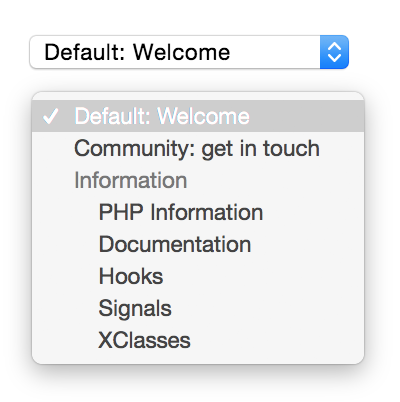
\includegraphics[width=0.3\linewidth]{ExtbaseFluid/62242.png}
	\end{figure}

\end{frame}

% ------------------------------------------------------------------------------
% LTXE-SLIDE-START
% LTXE-SLIDE-UID:		fcedda4d-c5f692fb-939dcebe-09d302fb
% LTXE-SLIDE-ORIGIN:	ea102c24-20cdb8de-eb67260a-af2a6967 English
% LTXE-SLIDE-ORIGIN:	44467f9a-abe64946-3da2bf4c-5bd094eb German
% LTXE-SLIDE-TITLE:		Feature/Breaking #63453: Template support for FlashMessagesViewHelper
% LTXE-SLIDE-REFERENCE:	Feature-63453-TemplateSupportForFlashMessagesViewHelper.rst
% LTXE-SLIDE-REFERENCE:	Breaking-63453-ChangedRenderingOfFlashMessagesViewHelper.rst
% ------------------------------------------------------------------------------

\begin{frame}[fragile]
	\frametitle{Extbase \& Fluid}
	\framesubtitle{Sjabloonondersteuning voor FlashMessagesViewHelper}

	% decrease font size for code listing
	\lstset{basicstyle=\tiny\ttfamily}

	\begin{itemize}

		\item De \texttt{FlashMessagesViewHelper} ondersteunt sjablonen

		\item Met het nieuwe attribuut \texttt{as} kan een variabelenaam ingesteld worden die gebruikt kan worden
			om binnen de onderliggende elementen van de ViewHelper de flash messages te benaderen

		\item Voorbeeld:

			\begin{lstlisting}
				<f:flashMessages as="flashMessages">
				  <ul class="myFlashMessages">
				    <f:for each="{flashMessages}" as="flashMessage">
				      <li class="alert {flashMessage.class}">
				        <h4>{flashMessage.title}</h4>
				        <span class="fancy-icon">{flashMessage.message}</span>
				      </li>
				    </f:for>
				  </ul>
				</f:flashMessages>
			\end{lstlisting}

		\item Let op: optie \texttt{renderMode} is deprecated

	\end{itemize}

\end{frame}

% ------------------------------------------------------------------------------
% LTXE-SLIDE-START
% LTXE-SLIDE-UID:		8e113115-86f49f38-3d47d7ff-0fac3ce1
% LTXE-SLIDE-ORIGIN:	3f5a8c27-78ff086f-99844ec0-a5e2d74a English
% LTXE-SLIDE-ORIGIN:	ec0810a7-c987f58a-9c42904e-8b7e0eba German
% LTXE-SLIDE-TITLE:		Feature #66111: Add TemplateRootPaths support to cObject FLUIDTEMPLATE (1)
% LTXE-SLIDE-REFERENCE:	Feature-66111-AddTemplaterootpathsSupportToCobjectFluidtemplate.rst
% ------------------------------------------------------------------------------

\begin{frame}[fragile]
	\frametitle{Extbase \& Fluid}
	\framesubtitle{Nieuwe eigenschappen van cObject \texttt{FLUIDTEMPLATE} (1)}

	\begin{itemize}

		\item cObject \texttt{FLUIDTEMPLATE} is uitgebreid met
			\texttt{templateRootPaths} en \texttt{templateName}

		\item Het is mogelijk om de naam van een sjabloon in te stellen en bij het renderen wordt dit sjabloon gebruikt
			samen met het ingesteld formaat om het sjabloon te vinden in de opgegeven
			\texttt{templateRootPaths}

		\item \texttt{templateRootPaths} biedt dezelfde fallback logica als
			\texttt{layoutRootPath} en \texttt{partialRootPath}

			\begin{itemize}
				\item templateName: string/stdWrap
				\item templateRootPaths: array van bestandspaden met ondersteuning voor "EXT:" prefix
			\end{itemize}

	\end{itemize}

\end{frame}

% ------------------------------------------------------------------------------
% LTXE-SLIDE-START
% LTXE-SLIDE-UID:		26ff1e3f-4e68cf12-2e4f77a2-c0f70229
% LTXE-SLIDE-ORIGIN:	90d6213a-883bc8d8-9c60e454-fac818a6 English
% LTXE-SLIDE-ORIGIN:	ec0810a7-c987f58a-9c42904e-8b7e0eba German
% LTXE-SLIDE-TITLE:		Feature #66111: Add TemplateRootPaths support to cObject FLUIDTEMPLATE (2)
% LTXE-SLIDE-REFERENCE:	Feature-66111-AddTemplaterootpathsSupportToCobjectFluidtemplate.rst
% ------------------------------------------------------------------------------

\begin{frame}[fragile]
	\frametitle{Extbase \& Fluid}
	\framesubtitle{Nieuwe eigenschappen van cObject \texttt{FLUIDTEMPLATE} (2)}

	% decrease font size for code listing
	\lstset{basicstyle=\tiny\ttfamily}

	\begin{itemize}

		\item TypoScript voorbeeld:

			\begin{lstlisting}
				lib.stdContent = FLUIDTEMPLATE
				lib.stdContent {
				  templateName = TEXT
				  templateName.stdWrap {
				    cObject = TEXT
				    cObject {
				      data = levelfield:-2,backend_layout_next_level,slide
				      override.field = backend_layout
				      split {
				        token = frontend__
				        1.current = 1
				        1.wrap = |
				      }
				    }
				    ifEmpty = Default
				  }
				  templateRootPaths {
				    10 = EXT:frontend/Resources/Private/Templates
				    20 = EXT:sitemodification/Resources/Private/Templates
				  }
				}
			\end{lstlisting}

	\end{itemize}

\end{frame}

% ------------------------------------------------------------------------------
% LTXE-SLIDE-START
% LTXE-SLIDE-UID:		d2e796c8-18d2f588-02a1bc85-c199a0b6
% LTXE-SLIDE-ORIGIN:	227004ec-e3e23728-e01cd083-cab72f98 English
% LTXE-SLIDE-ORIGIN:	5d3c259c-f79dd1fe-4f272783-a63cf715 German
% LTXE-SLIDE-TITLE:		Feature #66269: Fluid: Remove ViewHelper xmlns-attributes and specified html tag (1)
% LTXE-SLIDE-REFERENCE:	Feature-66269-FluidRemoveViewHelperXmlnsAttributesAndSpecifiedHtmlTag.rst
% ------------------------------------------------------------------------------

\begin{frame}[fragile]
	\frametitle{Extbase \& Fluid}
	\framesubtitle{Verwijderen van \texttt{xmlns}-attributen en HTML Tags (1)}

	% decrease font size for code listing
	\lstset{basicstyle=\tiny\ttfamily}

	\begin{itemize}

		\item Met de introductie van \texttt{xmlns:*} attributen om
			ViewHelpers in te voegen, is het mogelijk voor IDE's om Fluid sjablonen te ondersteunen.
			Het probleem is dat \texttt{xmlns:*} attributen en de overeenkomstige tag
			ook worden weergegeven wat meestal ongewenst is.

		\item Als workaround kunnen sections gebruikt worden, maar deze oplossing is niet vanzelfsprekend
			en niet beschikbaar in layouts. Ook geeft het meer werk bij de verwerking.

		\item \texttt{xmlns:*} attributen voor valide ViewHelper namespaces zullen nu verwijderd worden
			voordat het gerenderd wordt als ze de volgende syntax hebben:
			\small\texttt{http://typo3.org/ns/<phpNamespace>}\normalsize\newline
			(\texttt{xmlns} attributen voor namespaces die niet voor ViewHelpers zijn blijven bewaard)

	\end{itemize}

\end{frame}

% ------------------------------------------------------------------------------
% LTXE-SLIDE-START
% LTXE-SLIDE-UID:		19e758fa-bc025446-3c6ce6b1-9e68da4c
% LTXE-SLIDE-ORIGIN:	78a19608-9b89498f-d9a26bb5-11fb53c8 English
% LTXE-SLIDE-ORIGIN:	27834f27-5d3c259c-f79dd1fe-a63cf715 German
% LTXE-SLIDE-TITLE:		Feature #66269: Fluid: Remove ViewHelper xmlns-attributes and specified html tag (2)
% LTXE-SLIDE-REFERENCE:	Feature-66269-FluidRemoveViewHelperXmlnsAttributesAndSpecifiedHtmlTag.rst
% ------------------------------------------------------------------------------

\begin{frame}[fragile]
	\frametitle{Extbase \& Fluid}
	\framesubtitle{Verwijderen van \texttt{xmlns}-attributen en HTML Tags (2)}

	% decrease font size for code listing
	\lstset{basicstyle=\tiny\ttfamily}

	\begin{itemize}

		\item Neem ViewHelper namespaces op in de HTML tag en het
			\texttt{data-namespace-typo3-fluid="true"} attribuut om te voorkomen dat de hele
			HTML tag gerenderd wordt

			\begin{lstlisting}
				<html data-namespace-typo3-fluid="true"
				  xmlns:f="http://typo3.org/ns/TYPO3/CMS/Fluid/ViewHelpers"
				  xmlns:n="http://typo3.org/ns/GeorgRinger/News/ViewHelpers">

				  <f:if condition="{newsItem.title}">
				    <f:then>
				      <n:titleTag>{newsItem.title}</n:titleTag>
				    </f:then>
				    <f:else>
				      <n:titleTag>Nieuwsdetail</n:titleTag>
				    </f:else>
				  </f:if>

				</html>
			\end{lstlisting}

	\end{itemize}

\end{frame}

% ------------------------------------------------------------------------------
% LTXE-SLIDE-START
% LTXE-SLIDE-UID:		66e7c1d8-19b7b1e1-6b3a1ce3-dfeebe06
% LTXE-SLIDE-ORIGIN:	a1ef516c-669ded34-a2a6d664-f4d82d94 English
% LTXE-SLIDE-ORIGIN:	f79dd1fe-4f272783-a63cf715-5d3c259c German
% LTXE-SLIDE-TITLE:		Feature #66709: Add TemplateRootPaths support to Fluid/View/StandaloneView
% LTXE-SLIDE-REFERENCE:	Feature-66709-AddTemplateRootPathsSupportToFluidViewStandaloneView.rst
% ------------------------------------------------------------------------------

\begin{frame}[fragile]
	\frametitle{Extbase \& Fluid}
	\framesubtitle{Nieuwe methodes in Fluid-StandaloneView}

	% decrease font size for code listing
	\lstset{basicstyle=\tiny\ttfamily}

	\begin{itemize}

		\item StandaloneView is uitgebreid met
			\texttt{setTemplateRootPaths(\$templatePaths)} en
			\texttt{setTemplate(\$templateName, \$throwException = TRUE)}

		\item Zelfde functionaliteit als cObject \texttt{FLUIDTEMPLATE}

		\item Voorbeeld (maak e-mail van een sjabloon):

			\begin{lstlisting}
				$view = GeneralUtility::makeInstance(StandaloneView::class);
				$view->setLayoutRootPaths(array(GeneralUtility::getFileAbsFileName(
				  'EXT:my_extension/Resources/Private/Layouts')));
				$view->setPartialRootPaths(array(GeneralUtility::getFileAbsFileName(
				  'EXT:my_extension/Resources/Private/Partials')));
				$view->setTemplateRootPaths(array(GeneralUtility::getFileAbsFileName(
				  'EXT:my_extension/Resources/Private/Templates')));
				$view->setTemplate('Email/Notification');
				$emailBody = $view->render();
			\end{lstlisting}

	\end{itemize}

\end{frame}

% ------------------------------------------------------------------------------
% LTXE-SLIDE-START
% LTXE-SLIDE-UID:		1282a75e-e20db20e-70709081-cf16c122
% LTXE-SLIDE-ORIGIN:	95baf76c-31fd3f59-e0f9a716-5a5cc8cb English
% LTXE-SLIDE-ORIGIN:	f79da63cf-7834f272-d1fe715-5d3c259c German
% LTXE-SLIDE-TITLE:		Feature #66907: Add Data Processing to FLUIDTEMPLATE content object (1)
% LTXE-SLIDE-REFERENCE:	Feature-66907-AddDataProcessingToFluidTemplateContentObject.rst
% ------------------------------------------------------------------------------

\begin{frame}[fragile]
	\frametitle{Extbase \& Fluid}
	\framesubtitle{Gegevensverwerking voor \texttt{FLUIDTEMPLATE} cObject (1)}

	% decrease font size for code listing
	\lstset{basicstyle=\smaller\ttfamily}

	\begin{itemize}

		\item cObject \texttt{FLUIDTEMPLATE} is uitgebreid met \texttt{dataProcessing}

		\item Deze instelling kan gebruikt worden om een of meerdere processors toe te voegen
			voor het bewerken van de \texttt{\$data} variabele van het cObject dat momenteel afgehandeld wordt\newline
			(bijv. \texttt{tt\_content} of \texttt{page})

		\item Processor moet de interface \texttt{FluidTemplateDataProcessorInterface} implementeren moet de volgende
			functie bevatten:

			\begin{lstlisting}
				function process(array &$data, array $processorConfiguration,
				  array $configuration, StandaloneView $view) {
				    [...]
				}
			\end{lstlisting}

	\end{itemize}

\end{frame}

% ------------------------------------------------------------------------------
% LTXE-SLIDE-START
% LTXE-SLIDE-UID:		4b15df7b-2893078c-f73f4233-186423c5
% LTXE-SLIDE-ORIGIN:	34ef94b7-988b06b4-78e81c3a-81e45590 English
% LTXE-SLIDE-ORIGIN:	4f272783-a63cf715-5d3c259c-f79dd1fe German
% LTXE-SLIDE-TITLE:		Feature #66907: Add Data Processing to FLUIDTEMPLATE content object (2)
% LTXE-SLIDE-REFERENCE:	Feature-66907-AddDataProcessingToFluidTemplateContentObject.rst
% ------------------------------------------------------------------------------

\begin{frame}[fragile]
	\frametitle{Extbase \& Fluid}
	\framesubtitle{Gegevensverwerking voor \texttt{FLUIDTEMPLATE} cObject (2)}

	% decrease font size for code listing
	\lstset{basicstyle=\tiny\ttfamily}

	\begin{itemize}

		\item Voorbeeld:

			\begin{lstlisting}
				my_custom_ctype = FLUIDTEMPLATE
				my_custom_ctype {
				  templateRootPaths {
				    10 = EXT:your_extension_key/Resources/Private/Templates
				  }
				  templateName = CustomName
				  settings {
				    extraParam = 1
				  }
				  dataProcessing {
				    1 = Vendor\YourExtensionKey\DataProcessing\MyFirstCustomProcessor
				    2 = AnotherVendor\AnotherExtensionKey\DataProcessing\MySecondCustomProcessor
				    2 {
				      options {
				        myOption = SomeValue
				      }
				    }
				  }
				}
			\end{lstlisting}

	\end{itemize}

\end{frame}

% ------------------------------------------------------------------------------
